\documentclass{beamer}
%\beamertemplateshadingbackground{brown!70}{yellow!10}
\mode<presentation>
{
    %\usetheme{Warsaw}
    \usecolortheme{crane}
    % or ...

%    \setbeamercovered{transparent}
    % or whatever (possibly just delete it)
}
\setbeamertemplate{navigation symbols}{}
\setbeamertemplate{footline}[frame number]{}

\usepackage{tikz,pgfplots}
\pgfplotsset{compat=newest}
\usepackage{mathtools}
\usepackage{relsize}
\usepackage[utf8]{inputenc}
\usepackage{amssymb}
\usepackage{amsmath}
\usepackage{colortbl}
%\usepackage{multicol}
\usepackage{cancel}
\usepackage{multirow}
\usepackage{algorithm}
\usepackage{algorithmic}
\usepackage{xfrac}
\usepackage{forloop}% http://ctan.org/pkg/forloop
\AtBeginSection[]
{
\begin{frame}<beamer>
\frametitle{Outline}
\tableofcontents[currentsection]
\end{frame}
}

\def\opt{{\textsc{OPT}_k}}
\def\const{{\mathrm{const}}}
\def\nnz{{\mathrm{nnz}}}
\def\r{\sfrac{\sigma_{\w}^2}{\sigma_{\xib}^2}}
\def\rm{\sfrac{\sigma_{\xib}^2}{\sigma_{\w}^2}}
\def\cmark{\Green{\checkmark}}
\def\xmark{\Red{\large\sffamily x}}
\newcommand{\pdet}{{\mathrm{pdet}}}
\newcommand{\MSPE}[1] {{\mathrm{MSPE}\big[#1\big]}}
\newcommand{\MSE}[1] {{\mathrm{MSE}\big[#1\big]}}
\def\Poisson{{\operatorname{Poisson}}}
\def\PB{{\operatorname{PB}}}
\newcommand{\DP}[1]{\mathcal{DP}^{#1}}
\def\Ic{\mathcal{I}}
\def\Jc{\mathcal{J}}
\def\Mc{\mathcal M}
\def\Ec{\mathcal E}
\def\sr{{\mathrm{sr}}}
\def\ktd{{k^{\underline{d}}}}
\def\Det{{\mathrm{Det}}}
\def\detu{{\widecheck{\mathrm{Det}}_\mu^\gamma}}
\def\deto{{\widehat{\mathrm{Det}}_\mu^\gamma}}
\def\Zu{{\widecheck{Z}_\mu^{\gamma}}}
\def\Zo{{\widehat{Z}_\mu^{\gamma}}}
\def\Zun{{\widecheck{Z}_\mu^{\gamma_n}}}
\def\Zon{{\widehat{Z}_\mu^{\gamma_n}}}
\newcommand{\Er}{\mathrm{Er}}
\newif\ifDRAFT
\DRAFTtrue
\ifDRAFT
\newcommand{\marrow}{\marginpar[\hfill$\longrightarrow$]{$\longleftarrow$}}
\newcommand{\niceremark}[3]
   {\textcolor{red}{\textsc{#1 #2:} \marrow\textsf{#3}}}
\newcommand{\ken}[2][says]{\niceremark{Ken}{#1}{#2}}
\newcommand{\manfred}[2][says]{\niceremark{Manfred}{#1}{#2}}
\newcommand{\michael}[2][says]{\niceremark{Michael}{#1}{#2}}
\newcommand{\michal}[2][says]{\niceremark{Michal}{#1}{#2}}
\newcommand{\feynman}[2][says]{\niceremark{Feynman}{#1}{#2}}
%\usepackage[inline]{showlabels}
\else
\newcommand{\ken}[1]{}
\newcommand{\michael}[1]{}
\newcommand{\michal}[1]{}
\newcommand{\feynman}[1]{}
\fi
\newcommand{\norm}[1]{{\| #1 \|}}

\newcommand{\deff}{d_{\textnormal{eff}}}
\def\ee{\mathrm{e}}
\newcommand\mydots{\makebox[1em][c]{.\hfil.\hfil.}}
\def\Sd{\mathscr{S}_{\!d}}
\newcommand{\dx}{\dxy_{\!\cal X}}
\newcommand{\dxk}{\dxy_{\!\cal X}^k}
\newcommand{\dk}{\dxy^k}
\newcommand{\dxy}{\mathrm{D}}
\def\simiid{\overset{\textnormal{\fontsize{6}{6}\selectfont
i.i.d.}}{\sim}}
%\newcommand{\Dxy}{D_{\!\cal X\!,\cal Y}}
\def\vskx{{\mathrm{VS}_{\!\dx}^k}}
\def\vsk{{\mathrm{VS}_{\!D}^k}}
\def\vskxm{{\mathrm{VS}_{\!\dx}^{k-1}}}
\def\vskm{{\mathrm{VS}_{\!D}^{k-1}}}
\def\vsdx{{\mathrm{VS}_{\!\dx}^d}}
\def\vsd{{\mathrm{VS}_{\!D}^d}}
\newcommand{\vs}[1]{{\mathrm{VS}_{\!D}^{#1}}}
\newcommand{\sigd}{\boldsymbol\Sigma_{\!\dx}}
\def\wols{\w_{\mathrm{LS}}}
\def\wds{\boldsymbol\w_{\!D}^*}
\def\kd{K_{\!\dx}}

\def\poly{{\mathrm{poly}}}
\def\polylog{{\mathrm{polylog}}}
\def\DPP{{\mathrm{DPP}}}
\def\DPPcor{{\DPP_{\!\mathrm{cor}}}}
\def\DPPens{{\DPP_{\!\mathrm{ens}}}}
\newcommand{\DPPreg}[1]{{\DPP_{\!\mathrm{reg}}^{#1}}}
\def\Vol{{\mathrm{VS}}}
\def\Lev{{\mathrm{Lev}}}
\newcommand\todod[1]{\Red{\# DH: #1}}
\newcommand{\explain}[2]{\mathrel{\overset{\makebox[0pt]{\text{\tiny
#1}}}{#2}}}
\def\tot {{\mathrm{tot}}}
\def\checkmark{\tikz\fill[scale=0.4](0,.35) -- (.25,0) --
(1,.7) -- (.25,.15) -- cycle;}
\newcommand{\mnote}[1]{{\bf\large \Magenta{*}}\marginpar{\small \Magenta{#1}}}
\newcommand{\bnote}[1]{{\bf #1}}

\newcommand{\sqrtshort}[1]{{\sqrt{\white{\Big|}\!\!\smash{\text{\fontsize{9}{9}\selectfont$#1$}}}}}
\newenvironment{proofof}[2]{\par\vspace{2mm}\noindent\textbf{Proof of {#1} {#2}}\ }{\hfill\BlackBox}
\newcommand{\sets}[2]
{{\hspace{-0.3mm}[\hspace{-0.3mm}#1\hspace{-0.3mm}]\hspace{-0.3mm}\choose
\hspace{-0.3mm}#2\hspace{-0.3mm}}}
\DeclareMathOperator{\sgn}{\textnormal{sgn}}
\DeclareMathOperator{\adj}{\textnormal{adj}}
\def\Rb{{\mathbf{R}}}
\DeclareMathOperator{\ws}{\widetilde{\w}}
\newcommand{\inote}[1]{{\bf {#1}}}
\def\xib{\boldsymbol\xi}
\def\Sigmab{\mathbf{\Sigma}}
\def\Sigmabh{\widehat{\Sigmab}}
\def\Sigmabt{\widetilde{\Sigmab}}
\def\S{\mathbf{S}}
\def\T{\mathbf{T}}
\def\xt{\tilde{x}}
\def\xbt{\widetilde{\x}}
\def\xbh{\widehat{\x}}
\def\ubh{\widehat{\u}}
\def\dom {{\mathrm{dom}}}
\def\val {{\mathrm{val}}}
\def\out {{\mathrm{out}}}
\def\iin  {{\mathrm{iin}}}
\def\s {\mathbf{s}}
\def\q {\mathbf{q}}
\def\qt{\tilde{q}}
\def\itld {j}
\def\ubt {\tilde{\u}}
\def\n{\{1..n\}}
\def\cb {\mathbf{c}}
\def\cW{\mathcal W}
\def\Xt{\widetilde{X}}
\def\Dbt{\widetilde{\D}}
\def\xtb{\tilde{\mathbf{x}}}
\def\ytb{\tilde{\mathbf{y}}}
\def\Xtb{\widetilde{\mathbf{X}}}
\def\Xbb{\overline{\X}}
\def\Xb{{\bar{\X}}}
\def\ybb{\overline{\y}}
\def\f{{\mathbf{f}}}
\def\g{{\mathbf{g}}}
\def\fbb{{\overline{\f}}}
\def\fb{{\overline{f}}}
\def\Xc{\mathcal{X}}
\def\W{\mathbf W}
\def\L{\mathbf{L}}
\def\Rb{\mathbf R}
\def\Pc{\mathcal{P}}
\def\Nc{\mathcal{N}}
\def\Pt{\widetilde{P}}
\def\Hc{\mathcal{H}}
\def\Wc{\mathcal{W}}
\def\Cc{\mathcal{C}}
\def\p{\mathbf p}
%\def\r{\mathbf r}
\def\Y{\mathbf Y}
\def\H{\mathbf H}
\def\K{\mathbf K}
\def\Kh{\widehat{K}}
\def\Kbh{{\widehat{\K}}}
\def\Q{\mathbf Q}
\def\Qbar{{\bar{\mathbf Q}}}
\def\Ytb{\widetilde{\mathbf{Y}}}
\def\c{{n-d\choose s-d}}
\DeclareMathOperator{\Proj}{Proj}
\newcommand{\Span}{\mathrm{span}}
\newcommand{\ofsubt}[1]{\mbox{\scriptsize \raisebox{0.25pt}{$(#1)$}}}
%\raisebox{0.5pt}{$($}}#1\mbox{\tiny \raisebox{0.5pt}{$)$}}}
\newcommand{\ofsub}[1]{\mbox{\small \raisebox{0.0pt}{$(#1)$}}}
%\newcommand{\ofsubb}[1]{\mbox{\footnotesize \raisebox{0.5pt}{$(#1)$}}}
%\newcommand{\ofsub}[1]{(#1)}
%\newcommand{\ofsub}[1]{\mbox{\tiny$|$\hspace{-0.5pt}\raisebox{-0.5pt}{$#1$}}}
\newcommand{\of}[2]{{#1{\!\ofsub{#2}}}}
\newcommand{\oft}[2]{{#1{\!\ofsubt{#2}}}}
\newcommand{\fof}[2]{{#1({#2})}}
\newcommand{\yof}[2]{{#1{\ofsub{#2}}}}
%\newcommand{\yofb}[2]{{#1{\ofsubb{#2}}}}
\newcommand{\lazy}{FastRegVol}
\newcommand{\volsamp}{RegVol}

\newcommand{\Sm}{{S_{-i}}}
\newcommand{\Sp}{{S_{+i}}}
\ifx\BlackBox\undefined
\newcommand{\BlackBox}{\rule{1.5ex}{1.5ex}}  % end of proof
\fi
%\renewcommand{\dagger}{+}
\DeclareMathOperator*{\argmin}{\mathop{\mathrm{argmin}}}
\DeclareMathOperator*{\argmax}{\mathop{\mathrm{argmax}}}
\DeclareMathOperator*{\diag}{\mathop{\mathrm{diag}}}
\def\x{\mathbf x}
\def\y{\mathbf y}
\def\ybh{\widehat{\mathbf y}}
\def\ybb{\bar{\mathbf y}}
\def\xbb{\bar{\mathbf x}}
\def\yb{{\bar y}}
\def\ybt{\widetilde{\mathbf y}}
\def\yh{\widehat{y}}
\def\yhb{\widehat{\y}}
\def\yt{\widetilde{y}}
\def\z{\mathbf z}
\def\a{\mathbf a}
\def\b{\mathbf b}
\def\w{\mathbf w}
\def\v{\mathbf v}
\def\m{\mathbf m}
\def\wbh{\widehat{\mathbf w}}
\def\wh{\widehat{\mathbf w}}
\def\vbh{\widehat{\mathbf v}}
\def\wbt{\widetilde{\mathbf w}}
\def\e{\mathbf e}
\def\zero{\mathbf 0}
\def\one{\mathbf 1}
\def\u{\mathbf u}
\def\ubbar{\bar{\mathbf u}}
\def\f{\mathbf f}
\def\ellb{\boldsymbol\ell}

\def\X{\mathbf X}
\def\Xs{\widetilde{\X}}
\def\B{\mathbf B}
\def\A{\mathbf A}
\def\C{\mathbf C}
\def\U{\mathbf U}
\def\Ubt{\widetilde{\mathbf U}}
\def\Ubh{\widehat{\mathbf U}}
\def\Ubbar{\bar{\mathbf U}}
\def\F{\mathbf F}
\def\D{\mathbf D}
\def\V{\mathbf V}
\def\M{\mathbf M}
\def\Mh{\widehat{\mathbf M}}
%\def\S{\mathbf S}
\def\Stb{\widetilde{\mathbf{S}}}
\def\Sbh{\widehat{\mathbf{S}}}
\def\St{\widetilde{\S}}
\def\Sh{\widehat{S}}
\def\Sc{\mathcal{S}}
\def\Fc{\mathcal{F}}
\def\Vc{\mathcal{V}}
\def\Bc{\mathcal{B}}
\def\Dc{\mathcal{D}}
\def\Z{\mathbf Z}
\def\Zbh{\widehat{\mathbf Z}}
\def\Zbt{\widetilde{\mathbf Z}}
\def\Abh{\widehat{\mathbf A}}
\def\I{\mathbf I}
\def\Ic{\mathcal I}
\def\II{\mathbf {I \!\,I}}
%\def\II{\boldsymbol {\mathbb I}}
\def\A{\mathbf A}
\def\P{\mathbf P}
\def\Ph{\widehat{\mathbf P}}
\def\cP{\mathcal P}
\def\cR{\mathcal R}
\def\Xt{\widetilde{\mathbf{X}}}
\def\Xh{\widehat{\mathbf{X}}}
\def\Rh{\widehat{R}}
\def\Ot{\widetilde{O}}
\def\At{\widetilde{\A}}


\def\E{\mathbb E}
\def\R{\mathbb R}
\def\N{\mathbb N}
\def\Pr{\mathrm{Pr}}
%\def\C{\mathbb C}
\def\tr{\mathrm{tr}}
\def\Sbar{{\bar{S}}}
\def\cS{{\mathcal{S}}}
\def\Tbar{{\bar{T}}}
\def\Tt{{\widetilde{T}}}
\def\rank{\mathrm{rank}}
\def\Prob{\mathrm{Prob}}
\def\Var{\mathrm{Var}}
\def\Xinv{(\X^\top\X)^{-1}}
\def\XinvS{(\X_S\X_S^\top)^{-1}}
\def\ABinvS{(\A_S\B_S^\top)^{-1}}
\def\ABinv{(\A\B^\top)^{-1}}
\def\xinv{\x_i^\top\Xinv\x_i}
\def\Xinvr{(\lambda\I+\X_{-1}^\top\X_{-1})^{-1}}
\def\pdet{\mathrm{pdet}}
\newcommand{\vol}{\mathrm{vol}}
%\newcommand{\defeq}{:=}
\newcommand{\defeq}{\stackrel{\textit{\tiny{def}}}{=}}
\newcommand{\di}{{[d+1]_{-i}}}
\newcommand{\cov}{\mathrm{cov}}
\let\origtop\top
\renewcommand\top{{\scriptscriptstyle{\origtop}}} % this makes transpose not so big

\definecolor{silver}{cmyk}{0,0,0,0.3}
\definecolor{yellow}{cmyk}{0,0,0.9,0.0}
\definecolor{reddishyellow}{cmyk}{0,0.22,1.0,0.0}
\definecolor{black}{cmyk}{0,0,0.0,1.0}
\definecolor{darkYellow}{cmyk}{0.2,0.4,1.0,0}
\definecolor{orange}{cmyk}{0.0,0.7,0.9,0}
\definecolor{darkSilver}{cmyk}{0,0,0,0.1}
\definecolor{grey}{cmyk}{0,0,0,0.5}
\definecolor{darkgreen}{cmyk}{0.6,0,0.8,0}
\newcommand{\Red}[1]{{\color{red}  {#1}}}
\newcommand{\Purple}[1]{{\color{purple}  {#1}}}
\newcommand{\Magenta}[1]{{\color{magenta}{#1}}}
\newcommand{\Green}[1]{{\color{darkgreen}  {#1}}}
\newcommand{\Blue}[1]{\color{blue}{#1}\color{black}}
\newcommand{\Orange}[1]{\textcolor{orange}{#1}\color{black}}
\newcommand{\Brown}[1]{{\color{brown}{#1}\color{black}}}
\newcommand{\Grey}[1]{{\color{grey}{#1}\color{black}}}
\newcommand{\white}[1]{{\textcolor{white}{#1}}}
\newcommand{\yellow}[1]{{\textcolor{reddishyellow}{#1}}}
\newcommand{\darkYellow}[1]{{\textcolor{darkYellow}{#1}}}
\newcommand{\grey}[1]{{\textcolor{grey}{#1}}}

\DeclareMathOperator{\half}{\frac{1}{2}}

\ifx\proof\undefined
\newenvironment{proof}{\par\noindent{\bf Proof\ }}{\hfill\BlackBox\\[2mm]}
\fi

\ifx\theorem\undefined
\newtheorem{theorem}{Theorem}
\fi

\ifx\example\undefined
\newtheorem{example}{Example}
\fi

\ifx\condition\undefined
\newtheorem{condition}{Condition}
\fi
\ifx\property\undefined
\newtheorem{property}{Property}
\fi

\ifx\lemma\undefined
\newtheorem{lemma}{Lemma}
\fi

\ifx\proposition\undefined
\newtheorem{proposition}{Proposition}
\fi

\ifx\remark\undefined
\newtheorem{remark}{Remark}
\fi

\ifx\corollary\undefined
\newtheorem{corollary}{Corollary}
\fi

\ifx\definition\undefined
\newtheorem{definition}{Definition}
\fi

\ifx\conjecture\undefined
\newtheorem{conjecture}{Conjecture}
\fi

\ifx\axiom\undefined
\newtheorem{axiom}{Axiom}
\fi

\ifx\claim\undefined
\newtheorem{claim}{Claim}
\fi

\ifx\assumption\undefined
\newtheorem{assumption}{Assumption}
\fi

\ifx\condition\undefined
\newtheorem{condition}{Condition}
\fi

\renewcommand{\Xinv}{(\X^\top\X)^{-1}}
\renewcommand{\Xinvr}{(\lambda\I+\X_{-1}^\top\X_{-1})^{-1}}
\definecolor{lightyellow}{cmyk}{0,0,0.3,0.0}

\title[]{Minimax experimental design:\\
\small Bridging the gap between statistical and worst-case approaches to least squares regression}

\author[]{Micha{\l } Derezi\'{n}ski\\
  \textit{FODA Institute, UC Berkeley}\\[4mm]
\small Joint work with\\ Ken Clarkson, Michael Mahoney and Manfred Warmuth}

\date{{\large $\pi$}\,{\small .\,2019}}

\begin{document}

\begin{frame}
    \titlepage
\end{frame}

%\section{Overview}

\begin{frame}
  \frametitle{Classical experimental design}
  Consider $n$ parameterized experiments:
  $\x_1,\dots,\x_n\in\R^d$.\\
  Each experiment has a real random response $y_i$ such that:
  \begin{align*}
    y_i = \x_i^\top\w^* + \xi_i,\qquad \xi_i\sim\Nc(0,\sigma^2)
  \end{align*}
  \pause
\textbf{Goal:} Select $k\ll n$ experiments to best estimate $\w^*$
  \pause
\begin{columns}
\begin{column}{0.3\textwidth}
\\ \vspace{0.8cm}
Select $S=\{4,6,9\}$\\
\vspace{1cm}
Receive $y_4, y_6, y_9$
\end{column}
\begin{column}{0.5\textwidth}
\begin{center}
	\begin{tikzpicture}[scale=0.9]
          \draw [fill=brown!30] (-2,0) rectangle (0,3);
          \draw [color=black] (-2,2) -- (0,2);
          \draw (-2.25,2) node {\mbox{\footnotesize $\x_4^\top$}}; 
          \draw [color=black] (-2,1.5) -- (0,1.5);
          \draw (-2.25,1.5) node {\mbox{\footnotesize $\x_6^\top$}}; 
          \draw [color=black] (-2,0.5) -- (0,0.5);
          \draw (-2.25,0.5) node {\mbox{\footnotesize $\x_9^\top$}}; 
	   \draw (-2.5,3) node {$\X$}; 
           \draw [decorate,decoration={brace}] (-2,3.1) -- (0,3.1);
          \draw (-1,3.4) node {\mbox{\fontsize{8}{8}\selectfont $d$}}; 
            \draw [color=lightgray,line width =0.5mm] (1,0) -- (1,3);
            \draw [color=lightgray] (0.75,3) node {$\y$};
            \draw (0.75,2) node {\mbox{\footnotesize $y_4$}}; 
            \draw (1,2) node {.}; 
            \draw[mark=*,mark size=1.5pt] plot coordinates{(1,2)};
            \draw (0.75,1.5) node {\mbox{\footnotesize $y_6$}}; 
            \draw (1,1.5) node {.}; 
            \draw[mark=*,mark size=1.5pt] plot coordinates{(1,1.5)};
            \draw (0.75,0.5) node {\mbox{\footnotesize $y_9$}}; 
            \draw[mark=*,mark size=1.5pt] plot coordinates{(1,.5)};
	\end{tikzpicture}
\end{center}
\end{column}
\end{columns}

\end{frame}

\begin{frame}
  \frametitle{A-optimal design}
  Find an unbiased estimator $\wbh$ with smallest
  \textit{mean squared error}:
  \begin{align*}
    \min_{\wbh}\max_{\w^*}\quad
    \underbrace{\E_{\wbh}\big[\|\wbh-\w^*\|^2\big]}_{\mathrm{MSE}[\wbh]}\quad\text{subject
    to}\quad\E\big[\wbh\big]=\w^*\ \ \forall_{\w^*}
  \end{align*}
  \pause
Given \only<1-2>{every $y_1,\dots,y_n$}\only<3->{\Blue{set $\{y_i:\,i\in S\}$}}, the optimum is \textit{least squares}: \only<1-2>{$\wbh=\X^\dagger\y$}\only<3->{$\wbh=\X ^\dagger_{\Blue{S}}\y_{\Blue{S}}$}
  \begin{align*}
    \only<1-2>{\MSE{\X^\dagger\y}=\tr\big(\Var[\X^\dagger\y]\big)=\sigma^2\tr\big((\X^\top\X)^{-1}\big)}
    \only<3->{\MSE{\X^\dagger_{\Blue{S}}\y_{\Blue{S}}} = \tr\big(\Var[\X^\dagger_{\Blue{S}}\y_{\Blue{S}}]\big)=\sigma^2\tr\big((\X^\top_{\Blue{S}}\X_{\Blue{S}})^{-1}\big)}
  \end{align*}
  \pause\pause
  \vspace{-3mm}
  \begin{align*}
    \text{A-optimal design:}\quad \min_{S:\,|S|\leq k}\tr\big((\X_S^\top\X_S)^{-1}\big)
  \end{align*}
  \pause
  \vspace{4mm}
  
  \Red{
    Recall:\quad $y_i = \x_i^\top\w^* +
    \xi_i,\quad\xi_i\sim\Nc(0,\sigma^2)$
  }
\end{frame}

\begin{frame}
  \frametitle{A-optimal design: a simple guarantee}
  \textbf{Theorem} (Avron and Boutsidis, 2013)\\
  For any $\X$ and $k\geq d$   there is $S$ of size $k$ such that:
  \begin{align*}
\tr\big((\X_S^\top\X_S)^{-1}\big)\leq
    \frac{n-d+1}{k-d+1}\,\underbrace{\tr\big((\X^\top\X)^{-1}\big)}_{\text{(denoted
    $\phi$)}}
  \end{align*}
  \pause
  \only<1-3>{  \vspace{3mm}}
\only<4>{  \vspace{-2mm}}
  
  \textbf{Corollary} If $\y = \X\w^*+\xib$ where
  \only<1-3>{\Red{$\Var[\xib]=\sigma^2\I$ and $\E[\xib]=\zero$}}
  \only<4>{\!\!$\overbrace{\Red{\Var[\xib]=\sigma^2\I\text{ and
        }\E[\xib]=\zero}}^{\text{Is this necessary?}}$\,\,} then
  \begin{align*}
    \underbrace{\tr\big(\Var[\X_S^\dagger\y_S]\big)}_{\sigma^2 \tr((\X_S^\top\X_S)^{-1})} %{\mathrm{MSE}[\X_S^\dagger\y_S]}
\leq \sigma^2\,\frac{n\!-\!d\!+\!1}{k\!-\!d\!+\!1}\,\phi
\leq \underbrace{\tfrac{\phi}{k-d+1}}_{\epsilon}\cdot\underbrace{\tr\big(\Var[\xib]\big)}_{n\sigma^2}
  \end{align*}
  \pause
\begin{center}\fcolorbox{reddishyellow}{lightyellow}{
 \parbox{0.95\textwidth}{  
\centering$k=\Blue{d+\phi/\epsilon}$\quad and\quad
$\mathrm{MSE}[\X_S^\dagger\y_S]\leq \epsilon\cdot \tr(\Var[\xib])$
}}\end{center}
\pause
\end{frame}

\begin{frame}
  \frametitle{General response model}
  $\Fc_n$ - all random vectors in $\R^n$ with finite second moment
  \pause
  \begin{align*}
    \y&\in\Fc_n
\\  \w^*&\defeq  \argmin_\w \E_\y \big[\|\X\w-\y\|^2\big]
    =\X^\dagger\E[\y],
\\ \xib_{\y|\X}&\defeq \y-\X\w^* = \y-\X\X^\dagger\E[\y]
  \end{align*}
  \pause\vspace{3mm}

Two special cases:\vspace{2mm}
\pause
\begin{enumerate}
\item Statistical regression:\quad\quad\  $\E\big[\xib_{\y|\X}\big]=\zero$
  \pause
\item Worst-case regression:\quad $\Var\big[\xib_{\y|\X}\big]=\zero$
\end{enumerate}

\end{frame}

\begin{frame}
  \frametitle{Random experimental designs}
  \textbf{Definition.} \ \textit{Random experimental design}
  $(S,\wbh)$ of size $k$:
  \begin{enumerate}
    \item a random set variable $S\subseteq \{1..n\}$ such that
      $|S|\leq k$
    \item a (jointly with $S$) random function $\wbh:\R^{|S|}\rightarrow\R^d$
    \end{enumerate}
    \pause\vspace{6mm}
    
    \textit{Mean squared error} of a random experimental design
    $(S,\wbh)$:
    \begin{align*}
      \MSE{\wbh(\y_S)} = \E_{S,\wbh,\y}\big[\|\wbh(\y_S)-\w^*\|^2\big]
    \end{align*}
    \pause\vspace{3mm}

$\Wc_k(\X)$ - family of \textit{unbiased} random experimental designs $(S,\wbh)$:
    \begin{align*}
      \E_{S,\wbh,\y}\big[\wbh(\y_S)\big] = \underbrace{\X^\dagger\E[\y]}_{\w^*}
      \qquad \text{for all }\y\in\Fc_n
    \end{align*}
  \end{frame}

  \begin{frame}
    \frametitle{Main result}
%   Recall: $\X$ is an $n\times d$ matrix such that $\tr\big((\X^\top\X)^{-1}\big)=\phi$
    \begin{theorem}
For any $\epsilon>0$, there is a random experimental design $(S,\wbh)$
of size
\[k=\only<1>{O(d\log n+\phi/\epsilon)}\only<2->{O(\Blue{d}\log n\Blue{\,+\,\phi/\epsilon})}, \quad\text{where}\quad\phi=\tr\big((\X^\top\X)^{-1}\big),\]
such that $(S,\wbh)\in\Wc_k(\X)$ (unbiasedness) and for any $\y\in\Fc_n$
%$\E\big[\wbh(\y_S)\big]=\X^\dagger\E[\y]$, and
\begin{align*}
\mathrm{MSE}\big[\wbh(\y_S)\big] - \mathrm{MSE}\big[\X^\dagger\y\big]
  \leq \epsilon\cdot 
  \E\big[\|\xib_{\y|\X}\|^2\big]%\quad\text{and}\quad k= O(d\log n + \phi/\epsilon).
\end{align*}
\end{theorem}
\pause\vspace{4mm}

\textit{Toy example:} \quad$\Var[\xib_{\y|\X}]=\sigma^2\I$,\quad\ 
$\E[\xib_{\y|\X}]=\zero$
\pause\vspace{3mm}
\begin{enumerate}
  \item $\E\big[\|\xib_{\y|\X}\|^2\big]
    %\tr\big(\Var[\xib_{\y|\X}]\big) + \big\|\E[\xib_{\y|\X}]\big\|^2
    =\tr\big(\Var[\xib_{\y|\X}]\big)$
    \pause\vspace{1mm}
  \item $\MSE{\X^\dagger\y} %= \sigma^2\phi    %\leq \sigma^2k\epsilon\ll
    % \sigma^2n \epsilon
    = \frac\phi n\cdot \tr\big(\Var[\xib_{\y|\X}]\big)$
  \end{enumerate}
  % \pause\vspace{3mm}
  
  % So in this case $\mathrm{MSE}\big[\wbh(\y_S)\big]\leq
  % O(\epsilon) \cdot \tr\big(\Var[\xib_{\y|\X}]\big)$ as expected
\end{frame}

\begin{frame}
  \frametitle{Important special instances}
  \begin{enumerate}
  \item    \textit{Statistical regression:}\quad
    $\y = \X\w^*+\xib$,\quad $\E[\xib]=\zero$
    \begin{align*}
      \mathrm{MSE}\big[\wbh(\y_S)\big] -
      \mathrm{MSE}\big[\X^\dagger\y\big]\leq \epsilon\cdot\tr\big(\Var[\xib]\big)
    \end{align*}
    \pause\vspace{-5mm}
    \begin{itemize}
    \item Weighted regression:\quad\ 
      $\Var[\xib]=\mathrm{diag}\big([\sigma_1^2,\dots,\sigma_n^2]\big)$\\[2mm]
      \pause
      \item Generalized regression: $\Var[\xib]$ is
        arbitrary\\[2mm]
        \pause
        \item Bayesian regression: \quad \,$\w^*\sim\Nc(\zero,\I)$
        \end{itemize}
        \pause\vspace{5mm}
      \item \textit{Worst-case regression:}\quad $\y$ is any fixed vector in
        $\R^n$
        \pause
        \begin{align*}
      \E_{S,\wbh}\big[\|\wbh(\y_S)-\w^*\|^2\big]\leq \epsilon\cdot
          \|\y-\X\w^*\|^2
        \end{align*}
where $\w^*=\X^\dagger\y$
  \end{enumerate}
\end{frame}

\begin{frame}
  \frametitle{Minimax experimental design}
  \begin{definition}
    Minimax A-optimal value for experimental design:
\begin{align*}
R_k^*(\X)&\defeq 
  \min_{(S,\wbh)\in\Wc_k(\X)}\ \max_{\y\in\Fc_n\backslash\mathrm{Sp}(\X)}\,\frac{\mathrm{MSE}\big[\wbh(\y_S)\big]-
     \mathrm{MSE}\big[\X^\dagger\y\big]
  }{\E\big[\|\xib_{\y|\X}\|^2\big]}
\end{align*}
\end{definition}
\pause
\textbf{Fact.} \ $\X^\dagger\y$ is the \textit{minimum
  variance unbiased estimator} for $\Fc_n$:
\begin{align*}
  \text{if}\quad  \E_{\y,\wbh}\big[\wbh(\y)\big]
  &=\X^\dagger\E[\y]\quad\quad\,\forall_{\y\in\Fc_n}
\\ \text{then}\quad
  \Var\big[\wbh(\y)\big]&\succeq\Var\big[\X^\dagger\y\big]\quad \forall_{\y\in\Fc_n}
\end{align*}
\pause
\begin{itemize}
\item If \ $d\leq k\leq n$,\qquad\quad then \
  $R_k^*(\X)\in[0,\infty)$
    \pause
\item If \ $k\geq C\cdot d\log n$,\quad \,then \ $R_k^*(\X)\leq
  C\cdot\phi/k$\hfill for some $C$
\pause
\item If \ $k^2<\epsilon nd/3$,\qquad\ \,then \ $R_k^*(\X)\geq
    (1\!-\!\epsilon)\cdot\phi/k$\hfill for some $\X$
\end{itemize}
\end{frame}

\begin{frame}
  \frametitle{Alternative: mean squared \textit{prediction} error}
\textbf{Definition.}\quad    $\MSPE{\wbh} =
\E\big[\|\X(\wbh-\w^*)\|^2\big]$\quad (V-optimality)
\pause\vspace{5mm}
  \begin{theorem}
    There is $(S,\wbh)$ of size $k=O(\Blue{d\log n +d/\epsilon})$ s.t.~for
    any $\y\in\Fc_n$,
    \begin{align*}
\mathrm{MSPE}\big[\wbh(\y_S)\big] - \mathrm{MSPE}\big[\X^\dagger\y\big]
  \leq \epsilon\cdot 
  \E\big[\|\xib_{\y|\X}\|^2\big]
\end{align*}
\end{theorem}
\pause\vspace{3mm}

Follows from the MSE bound by reduction to $\X^\top\X=\I$. 
\begin{align*}
\text{Then}\quad\mathrm{MSPE}\big[\wbh\big]=\mathrm{MSE}\big[\wbh\big]\quad\text{and}\quad\phi=d.
\end{align*}
\pause\vspace{2mm}

Minimax V-optimal value:
\begin{align*}
\min_{(S,\wbh)\in\Wc_k(\X)}\ \max_{\y\in\Fc_n\backslash\mathrm{Sp}(\X)}\,\frac{\mathrm{MSPE}\big[\wbh(\y_S)\big]-
     \mathrm{MSPE}\big[\X^\dagger\y\big]
  }{\E\big[\|\xib_{\y|\X}\|^2\big]}
\end{align*}
\end{frame}


\begin{frame}
  \frametitle{Questions about minimax experimental design}
  \begin{enumerate}
  \item Can $R_k^*(\X)$ be found, exactly or approximately?\\[4mm]
    \pause
  \item What happens in the regime of $k\leq C\cdot d\log n$?\\[4mm]
    \pause
  \item
Can we restrict $\Wc_k(\X)$ to only tractable experimental designs?\\[4mm]
\pause
  \item Does the minimax-value change when you restrict $\Fc_n$?\\[1mm]
    \pause
    \begin{enumerate}
    \item Weighted regression\\[1mm]
    \item Generalized regression\\[1mm]
    \item Bayesian regression\\[1mm]
    \item Worst-case regression
      \end{enumerate}
  \end{enumerate}
\end{frame}

\begin{frame}
  \frametitle{Reduction to worst-case regression}
  \begin{theorem}
    W.l.o.g.~we can replace random $\y\in\Fc_n$ with fixed $\y\in\R^n$:
    \begin{align*}
R_k^*(\X)&=
  \min_{(S,\wbh)\in\Wc_k(\X)}\ \max_{\y\in\R^n\backslash\mathrm{Sp}(\X)}\,\frac{\E_{S,\wbh}\big[\|\wbh(\y_S)-\X^\dagger\y\|^2\big]
  }{\|\y-\X\X^\dagger\y\|^2}     
    \end{align*}
  \end{theorem}
  \pause  \vspace{4mm}
Suppose  $(S,\wbh)$ for all fixed response vectors $\y\in\R^n$ satisfies 
  \begin{align*}
    \E\big[\wbh(\y_S)\big]=\X^\dagger\y\quad\text{and}\quad
    \E\big[\|\wbh(\y_S)-\X^\dagger\y\|^2\big]\leq
    \epsilon\cdot\|\y-\X\X^\dagger\y\|^2.
  \end{align*}
  \pause
Then, for all random response vectors $\y\in \Fc_n$ and $\w^*\in\R^d$,
  \begin{align*}
    \underbrace{\E\big[\|\wbh(\y_S)-\w^*\|^2\big]}_{\mathrm{MSE}[\wbh(\y_S)]}
    \leq
    \underbrace{\E\big[\|\X^\dagger\y-\w^*\|^2\big]}_{\mathrm{MSE}[\X^\dagger\y]}
    \,+\,\epsilon\cdot \E\big[\|\y-\X\w^*\|^2\big].
  \end{align*}
\end{frame}

\begin{frame}
  \frametitle{Proof of reduction}
  Note that $\E\big[\wbh(\y_S)\mid\y\big]=\X^\dagger\y$ (unbiasedness) so
  \begin{align*}
\hspace{-4mm}\E\big[\|\wbh(\y_S)-\w^*\|\big]
    &= \E\Big[\E\big[\|\wbh(\y_S)-\X^\dagger\y +
      \X^\dagger\y -\w^*\|^2\mid\y\big]\Big]
    \\[1mm]
    \hspace{-4mm}\text{(unbiasedness)}\quad
    &=\E\Big[\E\big[\|\wbh(\y_S)-\X^\dagger\y\|^2\mid\y\big] +
    \E\big[\|\X^\dagger\y -\w^*\|^2\mid\y\big]\Big]
    \\[1mm]
    &=\underbrace{\E\big[\|\wbh(\y_S)-\X^\dagger\y\|^2\big]}_{\leq\,\epsilon\,\cdot\,\E_{\y}[ \|\y-\X\X^\dagger\y\|^2]} +
\E\big[\|\X^\dagger\y -\w^*\|^2\big]
  \end{align*}
  \pause
  \begin{align*}
    \E_{\y}\big[\|\y-\X\X^\dagger\y\|^2\big] =
    \E_{\y}\Big[\min_\w\|\y-\X\w\|^2\Big]\leq \underbrace{\E_{\y}\big[\|\y-\X\w^*\|^2\big]}_{\E[\|\xib_{\y|\X}\|^2]}
  \end{align*}
\end{frame}

\begin{frame}
  \frametitle{Main result: proof outline}
  \pause
  \begin{enumerate}
  \item Volume sampling:\\[1mm]\pause
    \begin{enumerate}
    \item well-conditioned matrices\\[1mm]\pause
    \item unbiased estimators\\[4mm]
    \end{enumerate}
    \pause
  \item Error bounds via i.i.d.~sampling:\\[1mm]\pause
    \begin{enumerate}
    \item leverage score sampling\\[1mm]\pause
    \item inverse score sampling\\[4mm]\pause
    \end{enumerate}
  \item Proving expected error bounds for least squares
  \end{enumerate}
\end{frame}

\begin{frame}
  \frametitle{Volume sampling}
\begin{definition}[[AB13{]}]
  \label{d:vs}
  Given a  full rank matrix  $\X\in\R^{n\times d}$ we define volume sampling
  $\Vol^k(\X)$ as a distribution over sets $S\subseteq [n]$ of size $k$:
  \begin{align*}
    \Pr(S) =
    \frac{\det(\X_S^\top\X_S)}{{n-d\choose k-d}\det(\X^\top\X)}.
  \end{align*}
\end{definition}
\vspace{5mm}
\pause
\begin{columns}
  \begin{column}{0.5\textwidth}
    Note: if $k=d$ then $\det(\X_S^\top\X_S)=\det(\X_S)^2$
$$
\Pr(S)\sim {\footnotesize
\begin{array}{l}
\text{\bf squared volume of parallelepiped} \\
\text{spanned by the $\{\x_i:i\in S\}$}
\end{array}
         }
$$
{\footnotesize Computational cost: $O(nd^2)$}
\end{column}
\begin{column}{.3\textwidth}
\only<1>{
\vspace{3.3cm}
}
\only<2->{
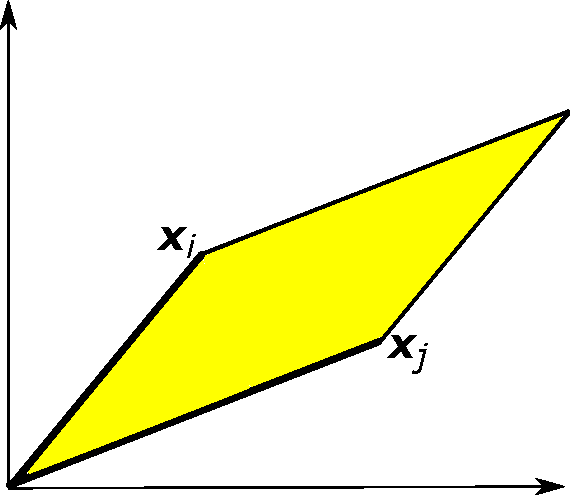
\includegraphics[width=\textwidth]{figs/volume_simple}
 }
\end{column}
\end{columns}
\end{frame}

\begin{frame}
  \frametitle{Volume sampling: well-conditioning}
  \begin{theorem}[[AB13,DW17{]}] 
    For any full rank $\X$, if $S\sim \Vol^k(\X)$ then:
    \begin{align*}
      \E\big[(\X_S^\top\X_S)^{-1}\big]\preceq \frac{n\!-\!d\!+\!1}{k\!-\!d\!+\!1}(\X^\top\X)^{-1}
    \end{align*}
  \end{theorem}
  \pause\vspace{5mm}
  
    \textit{Recall:} \ If $\y = \X\w^*+\xib$ where
    \Red{$\Var[\xib]=\sigma^2\I$ and $\E[\xib]=\zero$},
    \\ then we are done!\\[3mm]
\pause
    \textit{Note:} Here, estimator $\X_S^\dagger\y_S$ is unbiased
    because:
    \begin{align*}
      \E\big[\X_S^\dagger\underbrace{(\X_S\w^*+\xib_S)}_{\y_S}\big] =
      \E_S\Big[\X_S^\dagger\big(\X_S\w^*+\underbrace{\E_{\xib}[\xib_S\mid
      S]}_{\zero}\big)\Big] = \w^*
    \end{align*}
    \pause
    What about when $\E[\xib]\neq \zero$?
\end{frame}

\begin{frame}
  \frametitle{Volume sampling: unbiasedness}
  \begin{theorem}[[DWH18ab{]}] 
For any $\X$ and
  $q=(q_1,\dots,q_n)$, let
  $\{i_1,\dots,i_d\}\sim\Vol^d(\X)$ and $\tilde{\pi}\sim q^{k-d}$. Then
  $\pi=[i_1,\dots,i_d,\tilde{\pi}_1,\dots,\tilde{\pi}_{k-d}]$ satisfies:
\begin{align*}
  \E\big[(\S_\pi\X)^\dagger \S_\pi\big] &= \X^\dagger, \quad\text{where}\quad
    \S_\pi = \begin{bmatrix}\frac1{\sqrt{k q_{\pi_1}}}\e_{\pi_1}^\top\\
      \vdots\\\frac1{\sqrt{k q_{\pi_k}}}\e_{\pi_k}^\top\end{bmatrix}
    \in\R^{k\times n}. 
\end{align*}
\end{theorem}
\pause\vspace{1mm}

$\pi\sim\Vol^d(\X)\times q^{k-d}$ defines an unbiased estimator for any $\y$:
\begin{align*}
\wbh(\y_S) &= (\S_\pi\X)^ \dagger\S_\pi\y,\quad\text{ where }  S = \{\pi_1\}\cup\dots\cup\{\pi_k\},
  \\[2mm]
\onslide<3>{  \E\big[\wbh(\y_S)\big] &= \E\big[(\S_\pi\X)^\dagger \S_\pi\big]\E[\y]=\X^\dagger\E[\y]=\w^*}
\end{align*}


\end{frame}

\begin{frame}
  \frametitle{Towards an error bound}
  W.l.o.g.~assume that $\y\in\R^n$, $\w^*=\X^\dagger\y$ and $\xib=\y-\X\w^*$
  \begin{align*}
\hspace{-3mm}\MSE{\wbh(\y_S)}
    &=
    \E\Big[\big\|\overbrace{(\X^\top\S_\pi^\top\S_\pi\X_S)^{\dagger}\X^\top\S_\pi^\top\S_\pi}^{(\S_\pi\X)^\dagger\S_\pi}\y_S-\w^*\big\|^2\Big]
\\[2mm] &=    \E\Big[\big\|(\X^\top\S_\pi^\top\S_\pi\X)^{\dagger}\ \
     \X^\top\S_\pi^\top\S_\pi(\y-\X\w^*)\big\|^2\Big]
\\[2mm] &=\E\Big[\ \
     \big\|\ \ \underbrace{(\X^\top\S_\pi^\top\S_\pi\X)^{\dagger}\X^\top\X}_{\approx\,(\X^\top\X)^\dagger\X^\top\X\,=\,\I}\ \
     \underbrace{(\X^\top\X)^{-1}\X^\top\S_\pi^\top\S_\pi\xib}_{\approx\,\X^\dagger\xib\,=\,\zero}
     \ \ \big\|^2\ \ \Big]
  \end{align*}
  \pause\vspace{3mm}
  
  Both terms can be approximated with i.i.d.~sampling,\\
  but they require different distributions!
\end{frame}

\begin{frame}
  \frametitle{Leverage score sampling}
\begin{definition}
The $i$th \textbf{leverage score} of $\X$ is
defined as $\ell_i(\X)\defeq \x_i^\top(\X^\top\X)^{-1}\x_i$,
\end{definition}
\pause
\begin{theorem}[[Tro2012{]}]
If distribution $q$ is such that
$q_i\geq \beta\,\frac{\ell_i(\X)}{d}$ for all $i\in[n]$, then an i.i.d.~sample
$\pi\sim q^k$ for $k\geq C\frac d\beta\log
\frac d\delta$ w.p.~at least $1-\delta$ satisfies
\begin{align*}
\frac12\,\X^\top\X\preceq
  \underbrace{\frac1k\sum_{i=1}^k\frac1{q_{\pi_i}}\x_{\pi_i}\x_{\pi_i}^\top}_{\X^\top\S_\pi^\top\S_\pi\X}\preceq
  \frac32\,\X^\top\X. 
\end{align*}
\end{theorem}

\end{frame}

\begin{frame}
\frametitle{Inverse score sampling}
\begin{definition}
The $i$th \textbf{inverse score} of $\X$ is
defined as $v_i(\X)\defeq \x_i^\top(\X^\top\X)^{-2}\x_i$,
\end{definition}
\pause
\begin{lemma}
If distribution $q$ is such that
$q_i\geq \beta\,\frac{v_i(\X)}{\phi}$ for all $i\in[n]$, then an i.i.d.~sample
$\pi\sim q^s$ for any $\xib\in\R^n$ satisfies:
\begin{align*}
\E\big[\|\X^\dagger\S_\pi^\top\S_\pi\xib - \X^\dagger\xib\|^2\big]
  \leq \frac1{\beta k} \underbrace{\tr\big((\X^\top\X)^{-1}\big)}_{\|\X^\dagger\|_F^2}\,\|\xib\|^2.
\end{align*}
\end{lemma}
\end{frame}

\begin{frame}
  \frametitle{Controlling the tail of i.i.d.~sampling}
  Let $\pi\sim\Vol^d(\X)\times q^{k-d}$ for some $q$ (chosen later)
  \pause
  \begin{align*}
      \text{Define event $A$ as:}\quad
\frac1k\sum_{i=d+1}^k\frac1{q_{\pi_i}}\x_{\pi_i}\x_{\pi_i}^\top\
      \succeq\ \frac12\,\X^\top\X.  
  \end{align*}
  \pause\vspace{5mm}
  
    Apply law of total expectation:
    \begin{align*}
      \MSE{\wbh(\y_S)}
      &= \Pr(A)\,\E\big[\|\wbh(\y_S)-\w^*\|^2\mid
        A\big]
\\[1mm] &\quad+\Pr(\neg A)\,\E\big[\|\wbh(\y_S)-\w^*\|^2\mid \neg A\big]
    \end{align*}
\end{frame}

\begin{frame}
  \frametitle{When event $A$ succeeds}
  Assume that $q_i\geq \beta \,v_i(\X)$ for all $i\in[n]$
  \pause
\begin{align*}
\Pr(A)\,&\E\big[\|\wbh(\y_S)-\w^*\|^2\mid A\big]
\\ &=\Pr(A)\,\E\Big[\ \
     \big\|\
     \overbrace{(\X^\top\S_\pi^\top\S_\pi\X)^{\dagger}\X^\top\X}^{\preceq\,
     2\I}\quad
   \X^\dagger\S_\pi^\top\S_\pi\xib
\ \big\|^2\ \mid \ A\ \Big]
\\ &  \leq
     4\cdot\E\Big[\big\|\X^\dagger\S_\pi^\top\S_\pi\xib\big\|^2\Big]
\\ & \lesssim 4\,\frac\phi{\beta k}\cdot\|\xib\|^2
\end{align*}
\end{frame}

\begin{frame}
  \frametitle{When event $A$ fails}
  Assume that $q_i\geq \beta\, \frac1n$ for all $i\in [n]$ so that
  $\S_\pi^\top\S_\pi\preceq \frac n\beta \I$.
  \begin{align*}
    \E\big[\|\wbh(\y_S)-\w^*\|^2\mid \neg A\big]
    &\leq
    \E\big[\|(\S_\pi\X)^\dagger\S_\pi\|^2\mid\neg A\big]\,\|\xib\|^2
\\ &\leq  4n\,\E\big[\|(\S_\pi\X)^\dagger\|_F^2\mid\neg
     A\big]\,\|\xib\|^2
\\ &=4n\, \E\Big[\tr\big((\X^\top\S_\pi^\top\S_\pi\X)^{-1}\big)\mid\neg
     A\Big]\,\|\xib\|^2
    \\
\onslide<2->{    \text{(independence)}\quad&\leq
     4nk\,\E_{S_{\circ}\sim\Vol^d(\X)}\Big[\tr\big((\X_{S_\circ}^\top\X_{S_\circ})^{-1}\big)\Big]\,\|\xib\|^2
\\
    &\leq4n(n\!-\!d\!+\!1)k\,\tr\big((\X^\top\X)^{-1}\big)\,\|\xib\|^2
\\ &=\mathrm{poly}(n)\cdot\phi\,\|\xib\|^2}
  \end{align*}
  \pause\pause\vspace{2mm}
  
  If $q_i\geq \beta\,\ell_i(\X)$ and $k\geq C\cdot d\log
  \big(d\cdot\mathrm{poly}(n)\big)$, then
  \vspace{-2mm}
  \begin{align*}
    \Pr(\neg A)\leq  \frac1{\mathrm{poly(n)}}
  \end{align*}
\end{frame}

\begin{frame}
  \frametitle{Resulting mixture of i.i.d.~distributions}
  We use a mixture distribution $q$ for some $\beta_1+\beta_2+\beta_3=1$:
  \begin{align*}
    q_i = \beta_1\cdot \frac{v_i(\X)}\phi + \beta_2\cdot \frac1n + \beta_3\cdot\frac{\ell_i(\X)}d
  \end{align*}
  \pause\vspace{5mm}
  
  \textbf{Question:} What is the optimum distribution $q$?\\
  Can we compute it efficiently?
\end{frame}

\begin{frame}
  \frametitle{Conclusions}

  \begin{enumerate}
  \item Experimental design without any noise assumptions\\[5mm]
    \pause
  \item New minimax optimality criterion\\[5mm]
    \pause
  \item Many open questions remain
  \end{enumerate}
  
\end{frame}

\begin{frame}
  \centering\Large Thank you
\end{frame}



\end{document}
